\lab{One-dimensional Optimization}{One-dimensional Optimization}
\labdependencies{}
\objective{Most mathematical optimization problems involve estimating the minimizer(s) of a scalar-valued function.
Many algorithms for optimizing functions with a high-dimensional domain depend on routines for optimizing functions of a single variable.
There are many techniques for optimization in one dimension, each with varying degrees of precision and speed.
In this lab, we explore Newton's method and basins of attraction, and then we implement the secant method and apply it to the backtracking problem.
}

\section*{Iterative Methods} % ================================================

An \emph{iterative method} is an algorithm that must be applied repeatedly to obtain a result.
The general idea behind any iterative method is to make an initial guess at the solution to a problem, apply a few easy computations to better approximate the solution, use that approximation as the new initial guess, and repeat until done.
More precisely, let $F$ be some function used to approximate the solution to a problem.
Starting with an initial guess of $x_0$, compute
\begin{equation}x_{k+1} = F(x_k)\label{eq:iter-summary}\end{equation}
for successive values of $k$ to generate a sequence $(x_k)_{k=0}^\infty$ that hopefully converges to the true solution.
If the terms of the sequence are vectors, they are denoted by $\x_k$.

In the best case, the iteration converges to the true solution $x$, written $\lim_{k\rightarrow\infty} x_k = x$ or $x_k\rightarrow x$.
In the worst case, the iteration continues forever without approaching the solution.
In practice, iterative methods require carefully chosen \emph{stopping criteria} to guarantee that the algorithm terminates at some point.
The general approach is to continue iterating until the difference between two consecutive approximations is sufficiently small, and to iterate no more than a specific number of times.
That is, choose a very small $\epsilon > 0$ and an integer $N\in\mathbb{N}$, and update the approximation using (\ref{eq:iter-summary}) until either
\begin{equation} % Stopping Criteria.
    |x_k - x_{k-1}| < \epsilon
    \qquad \text{or} \qquad
    k > N.
\end{equation}

The choices for $\epsilon$ and $N$ are significant: a ``large'' $\epsilon$ (such as $10^{-6}$) produces a less accurate result than a ``small'' $\epsilon$ (such $10^{-16}$), but demands less computations; a small $N$ (10) also potentially lowers accuracy, but detects and halts nonconvergent iterations sooner than a large $N$ (10,000).
In code, $\epsilon$ and $N$ are often named \li{tol} and \li{maxiter}, respectively (or similar).

While there are many ways to structure the code for an iterative method, probably the cleanest way is to combine a \li{for} loop with a \li{break} statement.
As a very simple example, let $F(x) = \frac{x}{2}$.
This method converges to $x = 0$ independent of starting point.

\begin{lstlisting}
>>> F = lambda x: x / 2
>>> x0, tol, maxiter = 10, 1e-9, 8
>>> for k in range(maxiter):           # Iterate at most N times.
...     print(x0, end='  ')
...     x1 = F(x0)                      # Compute the next iteration.
...     if abs(x1 - x0) < tol:          # Check for convergence.
...         break                       # Upon convergence, stop iterating.
...     x0 = x1                         # Otherwise, continue iterating.
...
<<10  5.0  2.5  1.25  0.625  0.3125  0.15625  0.078125>>
\end{lstlisting}

In this example, the algorithm terminates after $N=8$ iterations (the maximum number of allowed iterations) because the tolerance condition $|x_k - x_{k-1}| < 10^{-9}$ is not met fast enough.
If $N$ had been larger (say $40$), the iteration would have quit early due to the tolerance condition.


\section*{Newton's Method} % ==================================================

\emph{Newton's method} is an important root-finding algorithm that can also be used for optimization.
Given $f:\mathbb{R}\rightarrow\mathbb{R}$ and a good initial guess $x_0$, the sequence $(x_k)_{k=1}^\infty$ generated by the recursive rule
\begin{equation}
    x_{k+1} = x_k - \frac{f(x_k)}{f'(x_k)}
    \label{eq:newton-1d-def}
\end{equation}
converges to a point $\bar{x}$ satisfying $f(\bar{x}) = 0$ as long as three conditions hold:
\begin{enumerate}
    \item $f$ and $f'$ exist and are continuous,
    \item $f'(\bar{x})\neq0$, and
    \item $x_0$ is ``sufficiently close'' to $\bar{x}$.
\end{enumerate}
In applications, the first two conditions usually hold.
If $\bar{x}$ and $x_0$ are not ``sufficiently close,'' Newton's method may converge very slowly, or it may not converge at all.
However, when all three conditions hold, Newton's method converges quadratically, meaning that the maximum error is squared at every iteration.
This is very quick convergence, making Newton's method as powerful as it is simple.


\begin{figure}[h] % Iterations of Newton's method.
    \centering
    \includegraphics[width=.7\textwidth]{figures/newton_iters.pdf}
    \caption{
    Newton's method approximates the zero of a function (blue) by choosing as the next approximation the $x$-intercept of the tangent line (red) that goes through the point $(x_k, f(x_k))$.
    In this example, $f(x) = e^x - 2$, which has a zero at $\bar{x} = \log(2)$.
    Setting $x_0 = 2$ and using \eqref{eq:newton-1d-def} to iterate, we have $x_1 = x_0 - \frac{f(x_0)}{f'(x_0)} = 2 - \frac{e^2 - 2}{e^2} \approx 1.2707$.
    Similarly, $x_2 \approx 0.8320$, $x_3 \approx .7024$, and $x_4 \approx 0.6932$.
    After only a few iterations, the zero $\log(2)\approx 0.6931$ is already computed to several digits of accuracy.}
    \label{fig:newton}
\end{figure}
    
\begin{problem}
\label{prob:newton-basic}
Write a function that accepts a function $f$, an initial guess \li{x0}, the derivative $Df$, a stopping tolerance \li{tol} defaulting to $10^{-5}$, and a maximum number of iterations \li{maxiter} defaulting to 15.
Use Newton's method as described in \eqref{eq:newton-1d-def} to compute a zero $\bar{x}$ of $f$.
Terminate the algorithm when $|x_k - x_{k-1}|$ is less than \li{tol} or after iterating \li{maxiter} times.
Return the last computed approximation to $\bar{x}$, a boolean value indicating whether or not the algorithm converged, and the number of iterations completed.

Test your function against functions like $f(x) = e^x - 2$ (see Figure \ref{fig:newton}) or $f(x) = x^4 - 3$.
Check that the computed zero $\bar{x}$ satisfies $f(\bar{x}) \approx 0$.
Also consider comparing your function to \li{scipy.optimize.newton()}, which accepts similar arguments.
\end{problem}

\begin{info}
Newton's method can be used to find zeros of functions that are hard to solve for analytically.
For example, the function $f(x) = \frac{\sin(x)}{x}-x$ is not continuous on any interval containing 0, but it can be made continuous by defining $f(0)=1$.
Newton's method can then be used to compute the zeros of this function.
\end{info}
    

\subsection*{Basins of Attraction} % ------------------------------------------

When a function $f$ has many zeros, the zero that Newton's method converges to depends on the initial guess $x_0$.
For example, the function $f(x)=x^2-1$ has zeros at $-1$ and $1$.
If $x_0<0$, then Newton's method converges to $-1$; if $x_0 > 0$ then it converges to $1$ (see Figure \ref{fig:basins-quadratic}).
The regions $(-\infty, 0)$ and $(0, \infty)$ are called the \emph{basins of attraction} of $f$.
Starting in one basin of attraction leads to finding one zero, while starting in another basin yields a different zero.

When $f$ is a polynomial of degree greater than 2, the basins of attraction are much more interesting.
For example, the basis of attraction for $f(x) = x^3-x$ are shown in Figure \ref{fig:basins-cubic}.
The basin for the zero at the origin is connected, but the other two basins are disconnected and share a kind of symmetry.

\begin{figure}[H] % 1-D basins of attraction.
\centering
\begin{subfigure}{.48\textwidth}
    \centering
    \includegraphics[width=\textwidth]{figures/basins_quadratic.pdf}
    \caption{Basins of attraction for $f(x) = x^2 -1$.}
    % With $\alpha=1$, blue values for $x_0$ converge to -1 and orange values converge to 1.}
    \label{fig:basins-quadratic}
\end{subfigure}
\quad
\begin{subfigure}{.48\textwidth}
    \centering
    \includegraphics[width=\textwidth]{figures/basins_cubic.pdf}
    \caption{Basins of attraction for $f(x) = x^3 -x$.}
        % With $\alpha=1$, blue values converge to $-1$, orange converge to 0, and green converge to 1.}
    \label{fig:basins-cubic}
\end{subfigure}
\caption{Basins of attraction with $\alpha=1$.
Since choosing a different value for $\alpha$ can change which zero Newton's method converges to, the basins of attraction may change for other values of $\alpha$.}
\end{figure}

It can be shown that Newton's method converges in any Banach space with only slightly stronger hypotheses than those discussed previously. % \footnote{See Chapter 7 of Volume 1 for details.}
In particular, Newton's method can be performed over the complex plane $\mathbb{C}$ to find imaginary zeros of functions.
Plotting the basins of attraction over $\mathbb{C}$ yields some interesting results.

The zeros of $f(x) = x^3 - 1$ are $1$, and $-\frac{1}{2} \pm \frac{\sqrt{3}}{2}i$.
To plot the basins of attraction for $f(x) = x^3-1$ on the square complex domain $X = \{a+bi \mid a \in [-\frac{3}{2},\frac{3}{2}], b \in [-\frac{3}{2},\frac{3}{2}]\}$,
create an initial grid of complex points in this domain using \li{np.meshgrid()}.
% Create the real and imaginary parts of the points separately, and then use \li{np.meshgrid()} to turn them into a single grid of complex numbers.

\begin{lstlisting}
>>> x_real = np.linspace(-1.5, 1.5, 500)    # Real parts.
>>> x_imag = np.linspace(-1.5, 1.5, 500)    # Imaginary parts.
>>> X_real, X_imag = np.meshgrid(x_real, x_imag)
>>> X_0 = X_real + 1j*X_imag                # Combine real and imaginary parts.
\end{lstlisting}

The grid $X_0$ is a $500\times500$ array of complex values to use as initial points for Newton's method.
Array broadcasting makes it easy to compute an iteration of Newton's method at every grid point.

\begin{lstlisting}
>>> f = lambda x: x**3 - 1
>>> Df = lambda x: 3*x**2
>>> X_1 = X_0 - f(X_0)/Df(X_0)
\end{lstlisting}

After enough iterations, the $(i,j)$th element of the grid $X_k$ corresponds to the zero of $f$ that results from using the $(i,j)$th element of $X_0$ as the initial point.
For example, with $f(x) = x^3 - 1$, each entry of $X_k$ should be close to $1$, $-\frac{1}{2} + \frac{\sqrt{3}}{2}i$, or $-\frac{1}{2} - \frac{\sqrt{3}}{2}i$.
Each entry of $X_k$ can then be assigned a value indicating which zero it corresponds to.
Some results of this process are displayed below.

\begin{figure}[H]
\centering
\begin{subfigure}{.49\textwidth}
    \centering
    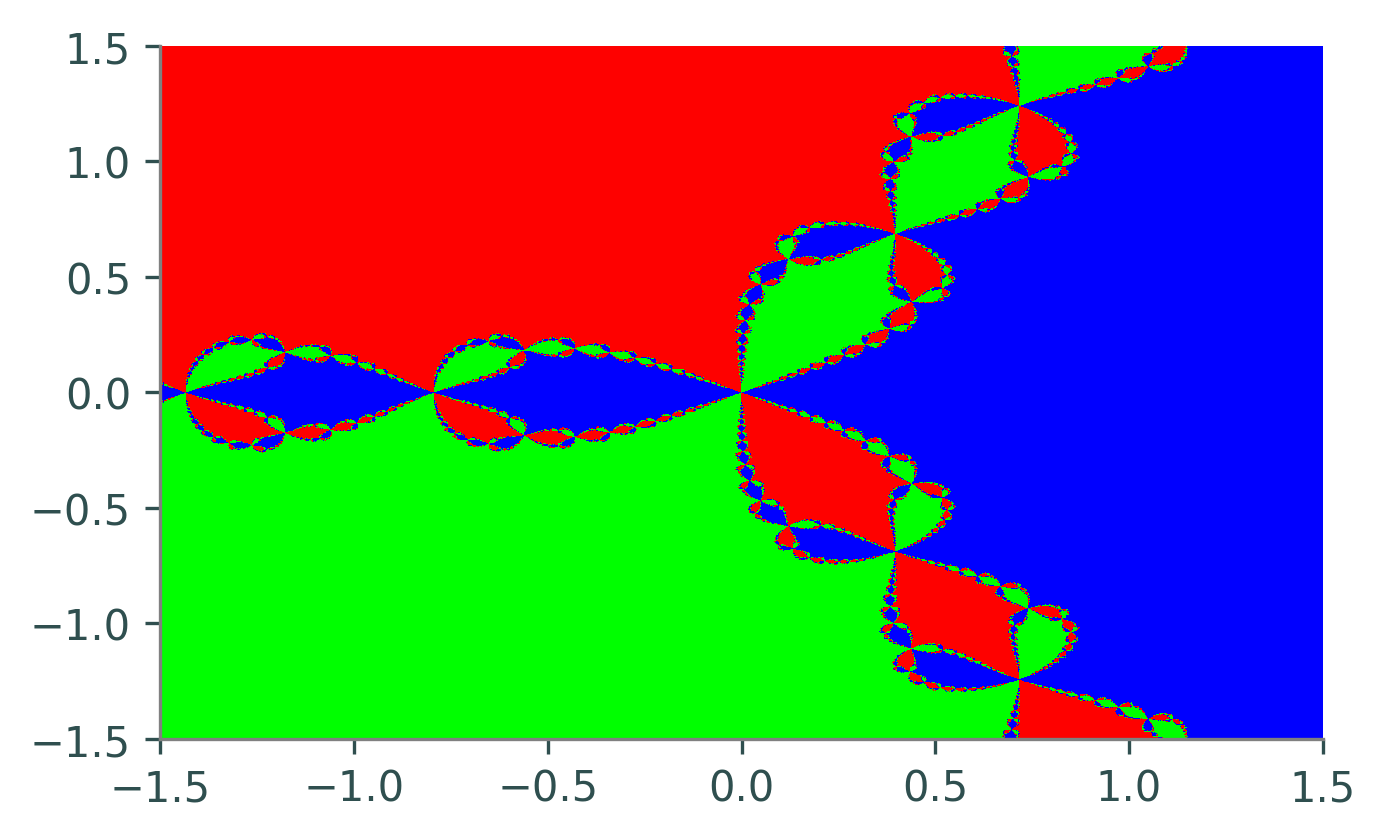
\includegraphics[width=\textwidth]{figures/fractal_hw.png}
    \caption{Basins of attraction for $f(x) = x^3-1$.}
    \label{fig:fractal_hw}
\end{subfigure}
\begin{subfigure}{.49\textwidth}
    \centering
    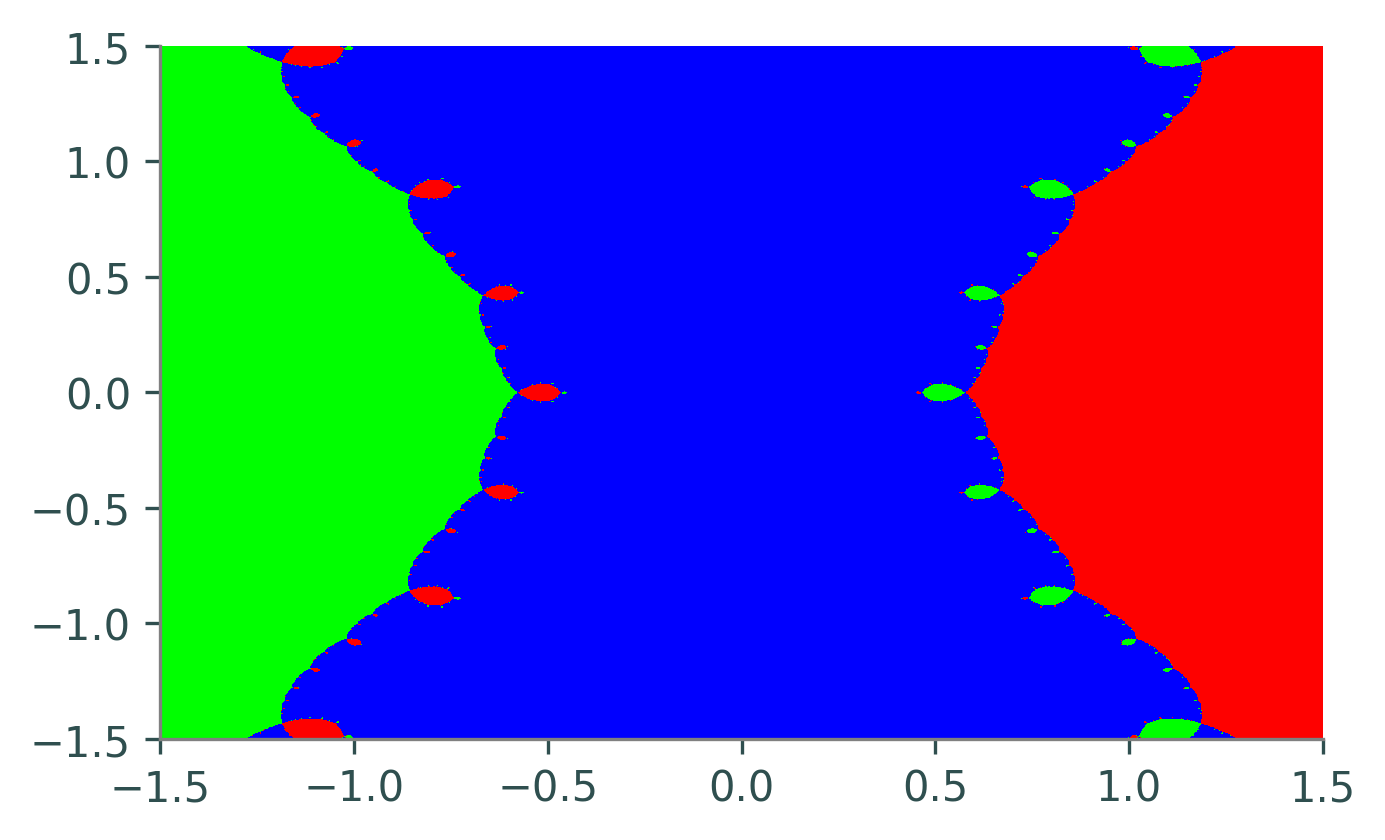
\includegraphics[width=\textwidth]{figures/fractal_ex.png}
    \caption{Basins of attraction for $f(x) = x^3-x$.}
    \label{fig:fractal_ex}
\end{subfigure}
\caption{}
\label{fig:newton-basins}
\end{figure}

\begin{info} % Newton fractals
Notice that in some portions of Figure \ref{fig:fractal_hw}, whenever red and blue try to come together, a patch of green appears in between.
This behavior repeats on an infinitely small scale, producing a fractal.
Because it arises from Newton's method, this kind of fractal is called a \emph{Newton fractal}.

Newton fractals show that the long-term behavior of Newton's method is \textbf{extremely} sensitive to the initial guess $x_0$.
Changing $x_0$ by a small amount can change the output of Newton's method in a seemingly random way.
This phenomenon is called \emph{chaos} in mathematics.
\end{info}

\begin{problem} % Plot the basins of attraction.
Write a function that accepts a function $f:\mathbb{C}\rightarrow\mathbb{C}$, its derivative $Df:\mathbb{C}\rightarrow\mathbb{C}$, an array \li{zeros} of the zeros of $f$, a list \li{domain} containing the bounds $[r_{\text{min}},r_{\text{max}},i_{\text{min}},i_{\text{max}}]$ for the domain of the plot, an integer \li{res} that determines the resolution of the plot, and number of iterations \li{iters} to run the iteration.
Compute and plot the basins of attraction of $f$ in the complex plane over the specified domain in the following steps.
\begin{enumerate}
\item Construct a \li{res}$\times$\li{res} grid $X_0$ over the domain $\{a+bi \mid a \in [r_{\text{min}},r_{\text{max}}], b \in [i_{\text{min}},i_{\text{max}}]\}$.

\item Run Newton's method on $X_0$ \li{iters} times, obtaining the \li{res}$\times$\li{res} array $x_{k}$.
Do not check for convergence at each step.
% To avoid the additional computation of checking for convergence at each step, do not use your function from Problem \ref{prob:newton-nd-implementation}.

\item $X_k$ cannot be directly visualized directly because its values are complex.
Solve this issue by creating another \li{res}$\times$\li{res} array $Y$.
To compute the $(i,j)$th entry $Y_{i,j}$, determine which zero of $f$ is closest to the $(i,j)$th entry of $X_k$.
Set $Y_{i,j}$ to the index of this zero in the array \li{zeros}.
If there are $R$ distinct zeros, each $Y_{i,j}$ should be one of $0,1,\ldots,R-1$.
\\(Hint: \li{np.argmin()} may be useful.)

\item Use \li{plt.pcolormesh()} to visualize the basins.
Recall that this function accepts three array arguments: the $x$-coordinates (in this case, the real components of the initial grid), the $y$-coordinates (the imaginary components of the grid), and an array indicating color values ($Y$).
Set \li{cmap="brg"} to get the same color scheme as in Figure \ref{fig:newton-basins}.
\end{enumerate}

Test your function using $f(x) = x^3-1$ and $f(x)=x^3-x$.
The resulting plots should resemble Figures \ref{fig:fractal_hw} and \ref{fig:fractal_ex}, respectively (perhaps with the colors permuted).
\end{problem}

\subsection*{The Secant Method} % ---------------------------------------------

The first-order necessary conditions from elementary calculus state that if $f$ is differentiable, then its derivative evaluates to zero at each of its local minima and maxima.
Therefore using Newton's method to find the zeros of $f'$ is a way to identify potential minima or maxima of $f$.
Specifically, starting with an initial guess $x_0$, set
\begin{equation}
    x_{k+1} = x_k - \frac{f'(x_k)}{f''(x_k)}
    \label{eq:1dopt-newton}
\end{equation}
and iterate until $|x_k - x_{k-1}|$ is satisfactorily small.
Note that this procedure does not use the actual function $f$ at all, but it requires many evaluations of its first and second derivatives.
As a result, Newton's method converges in few iterations, but it can be computationally expensive.

The second derivative of an objective function is not always known or may be prohibitively expensive to evaluate.
The \emph{secant method} solves this problem by numerically approximating the second derivative with a difference quotient.
\begin{equation*}
    f''(x) \approx \frac{f'(x + h) - f'(x)}{h}
\end{equation*}
Selecting $x = x_k$ and $h = x_{k-1} - x_k$ gives the following approximation.
\begin{equation}
    f''(x_k) \approx \frac{f'(x_k + x_{k-1} - x_k) - f'(x_k)}{x_{k-1} - x_k} = \frac{f(x_k) - f'(x_{k-1})}{x_k - x_{k-1}}
    \label{eq:1dopt-secant-approx}
\end{equation}
Inserting \eqref{eq:1dopt-secant-approx} into \eqref{eq:1dopt-newton} results in the complete secant method formula.
\begin{equation}
    x_{k+1}
    = x_k - \frac{x_k - x_{k-1}}{f'(x_k) - f'(x_{k-1})}f'(x_k)
    = \frac{x_{k-1}f'(x_k) - x_{k}f'(x_{k-1})}{f'(x_k) - f'(x_{k-1})}
    \label{eq:1dopt-secant-method}
\end{equation}
Notice that this recurrence relation requires two previous points (both $x_{k}$ and $x_{k-1}$) to calculate the next estimate.
This method converges superlinearly --- slower than Newton's method --- with convergence criteria similar to Newton's method.

\begin{problem} % Implement secant method.
Write a function that accepts a first derivative \li{df}, starting points \li{x0} and \li{x1}, a stopping tolerance \li{tol}, and a maximum of iterations \li{maxiter}.
Use \eqref{eq:1dopt-secant-method} to implement the Secant method.
Try to make as few computations as possible by only computing \li{df} at $(x_k)$ once for each $k$.
Return the minimizer approximation, whether or not the algorithm converged, and the number of iterations computed.

Test your code with the function $f(x) = x^2 + \sin(x) + \sin(10x)$ and with initial guesses of $x_0 = 0$ and $x_1 = -1$.
Plot your answer with the graph of the function.
Also compare your results to \li{scipy.optimize.newton()}; without providing the \li{fprime} argument, this function uses the secant method.
However, it still only takes in one initial condition, so it may converge to a different local minimum than your function.

\begin{lstlisting}
>>> df = lambda x: 2*x + np.cos(x) + 10*np.cos(10*x)
>>> optimize.newton(df, x0=0, tol=1e-10, maxiter=500)
2.3155516573790806
\end{lstlisting}
\end{problem}

\section*{Descent Methods} % ==================================================

Consider now a function $f:\mathbb{R}^n\rightarrow\mathbb{R}$.
% Minimizing $f$ is a \emph{high-dimensional optimization problem} because the domain of $f$ is $\mathbb{R}^n$ instead of $\mathbb{R}$.
\emph{Descent methods}, also called \emph{line search methods}, are optimization algorithms that create a convergent sequence $(x_k)_{k=1}^\infty$ by the following rule.
\begin{equation}
\x_{k+1} = \x_k + \alpha_k \textbf{p}_k
\end{equation}
Here $\alpha_k \in \mathbb{R}$ is called the \emph{step size} and $\textbf{p}_k \in \mathbb{R}^n$ is called the \emph{search direction}.
The choice of $\textbf{p}_k$ is usually what distinguishes an algorithm;
in the one-dimensional case ($n = 1$), $p_k = f'(x_k)/f''(x_k)$ results in Newton's method, and using the approximation in \eqref{eq:1dopt-secant-approx} results in the secant method.

To be effective, a descent method must also use a good step size $\alpha_k$.
If $\alpha_k$  is too large, the method may repeatedly overstep the minimum; if $\alpha_k$ is too small, the method may converge extremely slowly.
See Figure \ref{fig:1dopt-overstep}.

\begin{figure}[H]
    \centering
    \includegraphics[width=.7\textwidth]{figures/large_alpha.pdf}
    \caption{If the step size $\alpha_k$ is too large, a descent method may repeatedly overstep the minimizer.}
    \label{fig:1dopt-overstep}
\end{figure}

Given a search direction $\textbf{p}_k$, the best step size $\alpha_k$ minimizes the function $\phi_k(\alpha) = f(\x_k + \alpha\textbf{p}_k)$.
Since $f$ is scalar-valued, $\phi_k:\mathbb{R}\rightarrow\mathbb{R}$, so any of the optimization methods discussed previously can be used to minimize $\phi_k$.
However, computing the best $\alpha_k$ at every iteration is not always practical.
 % especially since computing a good $\mathbf{p}_k$ is generally more critical.
Instead, some methods use a cheap routine to compute a step size that may not be optimal, but which is good enough.
% These methods do not seek to minimize $\phi_k(\alpha)$, but instead seek to sufficiently decrease it.
The most common approach is to find an $\alpha_k$ that satisfies the \emph{Wolfe conditions}:
\begin{align}
&f(\textbf{x}_k + \alpha_k \textbf{p}_k) \leq f(\textbf{x}_k) + c_1\alpha_k Df(\textbf{x}_k)\trp \textbf{p}_k
\label{eq:1dopt-wolfe-armijo}
\\
& - Df(\textbf{x}_k + \alpha_k \textbf{p}_k)\trp \textbf{p}_k \leq -c_2 Df(\textbf{x}_k)\trp \textbf{p}_k
\label{eq:1dopt-wolfe-curvature}
\end{align}
where $0 < c1 < c2 < 1$ (for the  best results, choose $c1 << c2$).
The condition \eqref{eq:1dopt-wolfe-armijo} is also called the \emph{Armijo rule} and ensures that the step decreases $f$.
However, this condition is not enough on its own.
By Taylor's theorem,
\begin{equation*}
    f(\textbf{x}_k + \alpha_k \textbf{p}_k) = f(\textbf{x}_k) + \alpha_k Df(\textbf{x}_k)\trp \textbf{p}_k + \mathcal{O}(\alpha_k^2).
\end{equation*}
Thus, a very small $\alpha_k$ will always satisfy \eqref{eq:1dopt-wolfe-armijo} since $Df(\textbf{x}_k)\trp\textbf{p}_k < 0$ (as $\textbf{p}_k$ is a descent direction).
The condition \eqref{eq:1dopt-wolfe-curvature}, called the \emph{curvature condition}, ensures that the $\alpha_k$ is large enough for the algorithm to make significant progress.

It is possible to find an $\alpha_k$ that satisfies the Wolfe conditions, but that is far from the minimizer of $\phi_k(\alpha)$.
The \emph{strong Wolfe conditions} modify \eqref{eq:1dopt-wolfe-curvature} to ensure that $\alpha_k$ is near the minimizer.
\begin{equation*}
    | Df(\textbf{x}_k + \alpha_k \textbf{p}_k)\trp \textbf{p}_k| \leq c_2| Df(\textbf{x}_k)\trp \textbf{p}_k|
\end{equation*}
The \emph{Armijo--Goldstein conditions} provide another alternative to \eqref{eq:1dopt-wolfe-curvature}:
\begin{equation*}
    f(\textbf{x}_k) + (1 - c)\alpha_k Df(\textbf{x}_k)\trp \textbf{p}_k \leq f(\textbf{x}_k + \alpha_k\textbf{p}_k) \leq f(\textbf{x}_k) + c\alpha_k Df(\textbf{x}_k)\trp\textbf{p}_k,
\end{equation*}
where $0 < c < 1$.
These conditions are very similar to the Wolfe conditions (the right inequality is \eqref{eq:1dopt-wolfe-armijo}), but they do not require the calculation of the directional derivative $ Df(\textbf{x}_k + \alpha_k \textbf{p}_k)\trp\textbf{p}_k$.
% They perform as well as the Wolfe conditions in most situations, but are not well-matched for quasi-Newton methods with positive definite Hessians. % ?

\subsubsection*{Backtracking}

A \emph{backtracking line search} is a simple strategy for choosing an acceptable step size $\alpha_k$: start with an fairly large initial step size $\alpha$, then repeatedly scale it down by a factor $\rho$ until the desired conditions are satisfied.
The following algorithm only requires $\alpha$ to satisfy \eqref{eq:1dopt-wolfe-armijo}.
This is usually sufficient, but if it finds $\alpha$'s that are too small, the algorithm can be modified to satisfy \eqref{eq:1dopt-wolfe-curvature} or one of its variants.

\begin{algorithm}[H]
\begin{algorithmic}[1]
\Procedure{backtracking}{$f$,\ $Df$,\ $\x_k$,\ $\mathbf{p}_k$,\ $\alpha$,\ $\rho$,\ $c$}
    \State \texttt{Dfp} $\gets Df(\x_k)\trp\mathbf{p}_k$
        \Comment{Compute these values only once.}
    \State \texttt{fx} $\gets f(\x_k)$
    \While{$\big(f(\x_k + \alpha\mathbf{p}_k) >$ \texttt{fx} $+\ c\alpha$\texttt{Dfp}$\big)$}
        \State $\alpha \gets \rho\alpha$
    \EndWhile
    \Return $\alpha$
\EndProcedure
\end{algorithmic}
\caption{Backtracking using the Armijo Rule}
\label{Alg:opt1d-backtracking}
\end{algorithm}

\begin{problem}
Write a function that accepts a function $f:\mathbb{R}^n\rightarrow\mathbb{R}$, its derivative $Df:\mathbb{R}^n\rightarrow\mathbb{R}^n$, an approximate minimizer $\x_k$, a search direction $\textbf{p}_k$, an initial step length $\alpha$, and parameters $\rho$ and $c$.
Implement the backtracking method of Algorithm \ref{Alg:opt1d-backtracking}.
Return the computed step size.

The functions $f$ and $Df$ should both accept 1-D NumPy arrays of length $n$.
For example, if $f(x,y,z) = x^2 + y^2 + z^2$, then $f$ and $Df$ could be defined as follows.
\begin{lstlisting}
>>> f = lambda x: x[0]**2 + x[1]**2 + x[2]**2
>>> Df = lambda x: np.array([2*x[0], 2*x[1], 2*x[2]])
\end{lstlisting}

SciPy's \li{scipy.optimize.linesearch.scalar_search_armijo()} finds an acceptable step size using the Armijo rule.
It may not give the exact answer as your implementation since it decreases $\alpha$ differently, but the answers should be similar.
\begin{lstlisting}
>>> from scipy.optimize import linesearch
>>> from jax import numpy as jnp
>>> from jax import grad

# Get a step size for f(x,y,z) = x^2 + y^2 + z^2.
>>> f = lambda x: x[0]**2 + x[1]**2 + x[2]**2
>>> x = jnp.array([150., .03, 40.])         # Current minimizer guesss.
>>> p = jnp.array([-.5, -100., -4.5])       # Current search direction.
>>> phi = lambda alpha: f(x + alpha*p)      # Define phi(alpha).
>>> dphi = grad(phi)
>>> alpha, _ = linesearch.scalar_search_armijo(phi, phi(0.), dphi(0.))
\end{lstlisting}
\end{problem}

\begin{comment} % This is a little too confusing

\newpage

\section*{Additional Material} % ==============================================

\subsection*{Golden Search Derivations} % -------------------------------------

The ratio of the lengths of $[a, \tilde{a}]$ and $[\tilde{a}, b]$ is the same as the ratio between the lengths of $[\tilde{a}, b]$ and $[a, b]$ as follows:
\begin{align*}
\frac{\tilde{a}-a}{b-\tilde{a}} &= \frac{(b-a)(1-\frac{1}{\varphi})}{b-b+\frac{b-a}{\varphi}} \\
&= \varphi(1-\frac{1}{\varphi}) \\
\frac{b-\tilde{a}}{b-a} &= \frac{1}{\varphi}
\end{align*}
As one of the properties of the golden ratio states that $\frac{1}{\varphi^2} = 1 - \frac{1}{\varphi}$, they are equal.

Chosing the test points according to the golden ratio saves on computations.
For example, consider the case where $f(\tilde{a}) > f(\tilde{b})$ and label $a_0 = a$ and $a_1 = \tilde{a}$.
Thus, $x^* \in [\tilde{a}, b]$ and for the next iteration
\begin{align*}
\tilde{a_1} &= b - \frac{b - a_1}{\varphi} \\
&= b - \frac{b - b + \frac{b - a_0}{\varphi}}{\varphi}\\
&= b - \frac{b - a_0}{\varphi^2}\\
&= a_0 + \frac{b - a_0}{\varphi}\\
&= \tilde{b}
\end{align*}
Therefore, the next $\tilde{a}$ is the previous $\tilde{b}$.
Similarly, if $f(\tilde{a}) < f(\tilde{b})$, then the next $\tilde{b}$ will be the previous $\tilde{a}$.
\end{comment}
